%%%%%%%%%%%%%%%%%%%%%%%%%%%%%%%%%%%%%%%%%%%%%%%%%%%
%
%  New template code for TAMU Theses and Dissertations starting Fall 2016.  
%
%
%  Author: Sean Zachary Roberson
%  Version 3.16.10
%  Last Updated: 9/29/2016
%
%%%%%%%%%%%%%%%%%%%%%%%%%%%%%%%%%%%%%%%%%%%%%%%%%%%

\documentclass[12pt]{report}

%These next lines change the font. Fixes for certain
%fonts will be implemented in a future release.

%Comment this line if you do not wish to use Times
%New Roman. The font used will then be the LaTeX
%default of Computer Modern.
\usepackage{times}
%\usepackage{cmbright}
\usepackage[T1]{fontenc}

%Do not change these settings. The geometry package
%Adjusts the margins to those specified by the Thesis
%Manual. 
\usepackage[letterpaper]{geometry}
\geometry{verbose,tmargin=1.25in,bmargin=1.25in,lmargin=1.4in,rmargin=1.15in}
 \usepackage[doublespacing]{setspace}
 \usepackage{tocloft}
 \usepackage[rm, tiny, center, compact]{titlesec}
 \usepackage{indentfirst}
 \usepackage{etoolbox}

\usepackage{tocvsec2}
 \usepackage[titletoc]{appendix}
 \usepackage{appendix}
 \usepackage{tamuconfig}

\usepackage{rotating}

%These are common AMS packages. Many LaTeX documents
%have these packages declared in their preambles.
\usepackage{amsmath, amsthm}

%This package allows for the use of graphics in the
%document.
\usepackage{graphicx}

%If you have JPEG format images, add .jpg as an
%allowed file extension below. Same for Bitmaps (.bmp).
\DeclareGraphicsExtensions{.png}

%It is best practice to keep all your pictures in
%one folder inside the main directory in which your
%TeX file is kept. Here the folder is named "graphic."
%Replace the name here with your folder's name, if needed.
%The period is needed due to relative referencing.
\graphicspath{ {./graphic/} }

%If needed, this will allow you to add the word "Page"
%to extra pages on your front matter lists.
\usepackage{afterpage}

%This is from the mdwtools package; it fixes some
%footnote commands and allows you to have footnotes in
%tables via the savenotes environment.
\usepackage{footnote}


% Added to fix issues with pdf searching in some versions of LaTeX
%\usepackage[T1]{fontenc}\usepackage{lmodern}
%%%%%%%%%%%%%%%%%%%%%%%%%%%%%

% Hyperref setup below.  You should be able to get away with using uncommenting just the first line.
%\usepackage[hidelinks]{hyperref}

% if \usepackage[hidelinks]{hyperref} doesn't work try this.
% \usepackage{hyperref}  % Hidelinks is an option that removes link visiability.  TAMU Thesis Offices prefers to not see the links. But often doesn't work.  
% 
% \hypersetup{
%     colorlinks=true,
%     linkcolor=black,
%     citecolor=black,
%     filecolor=black,
%     urlcolor=black,
% }
%%%%%%%  End of hyperref setup.  One of these two options should work, but my motto with hyperref is when in doubt, comment it out!
%%%%%%%%%  This hopefully fixes the problem with vertical spacing of section headings at the top of the page..  Commented out in 1.0.7
% \preto\section{%
% \ifnum\value{section}>0\addtocontents{toc}{\vskip-6pt}\fi
% }
% \preto\subsection{%
% \ifnum\value{subsection}=0\addtocontents{toc}{\vskip-6pt}\fi
% \ifnum\value{subsection}>0\addtocontents{toc}{\vskip-6pt}\fi
% } 
%%%%%%%%%%%%%%%%%%%%%%%%%%%%%%%%%%%%%%%%%%%%%%%%%%%%%%

\begin{document}

%The title of your document goes here.
%Spacing may need to be adjusted if your title is long
%and pushes the copyright off the page.
\renewcommand{\tamumanuscripttitle}{Machine Learning for Anomaly Detection in Overlapping Aerial Image Streams}

%Type only Thesis, Dissertation, or Record of Study.
\renewcommand{\tamupapertype}{Thesis}

%Your full name goes here, as it is in university records. Check your student record on Howdy if there is any mismatch.
\renewcommand{\tamufullname}{Travis Taghavi}

%The degree title goes here. See the OGAPS site for more info.
\renewcommand{\tamudegree}{Master of Science}
\renewcommand{\tamuchairone}{Dr. Jean-Francois Chamberland}


% Uncomment out the next line if you have co-chairs.  You will also need to edit the titlepage.tex file.
%\newcommand{\tamuchairtwo}{Additional Chair Name}
\renewcommand{\tamumemberone}{Dr. Gregory Huff}
\newcommand{\tamumembertwo}{Dr. Krishna Narayanan}
\newcommand{\tamumemberthree}{Dr. Dylan Shell}
\renewcommand{\tamudepthead}{Dr. M. Begovic}

%Type only May, August, or December.
\renewcommand{\tamugradmonth}{August}
\renewcommand{\tamugradyear}{2017}
%Your department name goes here.
\renewcommand{\tamudepartment}{Electrical Engineering}


%%%%%%%%%%%%%%%%%%%%%%%%%%%%%%%%%%%%%%%%%%%%%%%%%%%
%
%  New template code for TAMU Theses and Dissertations starting Fall 2016.  
%
%
%  Author: Sean Zachary Roberson
%	 Version 3.16.09
%  Last updated 9/12/2016
%
%%%%%%%%%%%%%%%%%%%%%%%%%%%%%%%%%%%%%%%%%%%%%%%%%%%

%%%%%%%%%%%%%%%%%%%%%%%%%%%%%% 
%% TITLE PAGE
%% The values get updated automatically.  Please do not make changes to this file other than adding/deleting committee members where necessary.
%%%%%%%%%%%%%%%%%%%%%%%%%%%%%%

\providecommand{\tabularnewline}{\\}



\begin{titlepage}
\begin{center}
\MakeUppercase{\tamumanuscripttitle}
\vspace{4em}

A \tamupapertype

by

\MakeUppercase{\tamufullname}

\vspace{4em}

\begin{singlespace}

Submitted to the Office of Graduate and Professional Studies of \\
Texas A\&M University \\

in partial fulfillment of the requirements for the degree of \\
\end{singlespace}

\MakeUppercase{\tamudegree}
\par\end{center}
\vspace{2em}
\begin{singlespace}
\begin{tabular}{ll}
 & \tabularnewline
& \cr
% If you have Co-Chairs comment out the 'Chair of Committee' line below and uncomment the 'Co-Chairs of Committee' line.
Chair of Committee, & \tamuchairone\tabularnewline
%Co-Chairs of Committee, & \tamuchairone\tabularnewline & \tamuchairtwo\tabularnewline
Committee Members, & \tamumemberone\tabularnewline
 & \tamumembertwo\tabularnewline
 & \tamumemberthree\tabularnewline
 & \tamumemberfour\tabularnewline
Head of Department, & \tamudepthead\tabularnewline

\end{tabular}
\end{singlespace}
\vspace{3em}

\begin{center}
\tamugradmonth \hspace{2pt} \tamugradyear

\vspace{3em}

Major Subject: \tamudepartment \par
\vspace{3em}
Copyright \tamugradyear \hspace{.5em}\tamufullname 
\par\end{center}
\end{titlepage}
\pagebreak{}




 % This is simply a file that formats and adds your titlepage, please do not edit this unless you have a specific need. .
%%%%%%%%%%%%%%%%%%%%%%%%%%%%%%%%%%%%%%%%%%%%%%%%%%%
%
%  New template code for TAMU Theses and Dissertations starting Fall 2016.  
%
%  Author: Sean Zachary Roberson
%	 Version 3.16.09
%  Last updated 9/12/2016
%
%%%%%%%%%%%%%%%%%%%%%%%%%%%%%%%%%%%%%%%%%%%%%%%%%%%
%%%%%%%%%%%%%%%%%%%%%%%%%%%%%%%%%%%%%%%%%%%%%%%%%%%%%%%%%%%%%%%%%%%%%
%%                           ABSTRACT 
%%%%%%%%%%%%%%%%%%%%%%%%%%%%%%%%%%%%%%%%%%%%%%%%%%%%%%%%%%%%%%%%%%%%%

\chapter*{ABSTRACT}
\addcontentsline{toc}{chapter}{ABSTRACT} % Needs to be set to part, so the TOC doesnt add 'CHAPTER ' prefix in the TOC.

\pagestyle{plain} % No headers, just page numbers
\pagenumbering{roman} % Roman numerals
\setcounter{page}{2}

\indent This thesis work is an exploration into the application of machine learning to a current problem relating to streams of aerial images, with application to hyperspectral or multistpectral images.
Multispectral or hyperspectral images contain information from outside the visible light spectrum, generally, in addition to capturing the visible light spectrum, with the latter containing more bands.
The streams of images referred to are taken by a unmanned aerial vehicle, UAV, over some space of land.

Our problem relates to flight inconsistencies in the UAV.
In an ideal scenario, our UAV captures a set of images from a specified height, pointed normally at the ground, with a predetermined amount of overlap between images.
However, due to inconsistencies inherent in most flight, the UAV will occasionally tilt or swing in such a way that the images captured are not in line with adjacent images, i.e. they do not have the required amount of overlap, and their information may be blurred.
This creates a problem when attempting image stitching afterwards, as such anomalous images will be irrecconcilable with adjacent images.
The goal here is to create a system which can, in pseudo-real time, detect images which are out of line, through the use of feature extraction and machine learning, so that they can be discarded and possibly recaptured.

Our research compares and evaluates a number of image features and learning algorithms on the basis of their performance in this task.
Further auxillary research relates more specifically to the content of the images, and includes image segmentation and clustering based on spectral signatures, as well as possible projection and illumination correction.


 

\pagebreak{}

%%%%%%%%%%%%%%%%%%%%%%%%%%%%%%%%%%%%%%%%%%%%%%%%%%%%
%
%  New template code for TAMU Theses and Dissertations starting Fall 2016.  
%
%  Author: Sean Zachary Roberson
%	 Version 3.16.09
%  Last updated 9/12/2016
%
%%%%%%%%%%%%%%%%%%%%%%%%%%%%%%%%%%%%%%%%%%%%%%%%%%%

%%%%%%%%%%%%%%%%%%%%%%%%%%%%%%%%%%%%%%%%%%%%%%%%%%%%%%%%%%%%%%%%%%%%%%
%%                           DEDICATION
%%%%%%%%%%%%%%%%%%%%%%%%%%%%%%%%%%%%%%%%%%%%%%%%%%%%%%%%%%%%%%%%%%%%%
\chapter*{DEDICATION}
\addcontentsline{toc}{chapter}{DEDICATION}  % Needs to be set to part, so the TOC doesnt add 'CHAPTER ' prefix in the TOC.



\begin{center}
\vspace*{\fill}
To my mother, my father, my grandfather, and my grandmother. To see what happens with multiple lines, I extend this next part into a second line.
\vspace*{\fill}
\end{center}

\pagebreak{}

%%%%%%%%%%%%%%%%%%%%%%%%%%%%%%%%%%%%%%%%%%%%%%%%%%%%
%
%  New template code for TAMU Theses and Dissertations starting Fall 2016.
%
%  Author: Sean Zachary Roberson
%	 Version 3.16.09
%  Last updated 9/12/2016
%
%%%%%%%%%%%%%%%%%%%%%%%%%%%%%%%%%%%%%%%%%%%%%%%%%%%


%%%%%%%%%%%%%%%%%%%%%%%%%%%%%%%%%%%%%%%%%%%%%%%%%%%%%%%%%%%%%%%%%%%%%%
%%                           ACKNOWLEDGMENTS
%%%%%%%%%%%%%%%%%%%%%%%%%%%%%%%%%%%%%%%%%%%%%%%%%%%%%%%%%%%%%%%%%%%%%
\chapter*{ACKNOWLEDGMENTS}
\addcontentsline{toc}{chapter}{ACKNOWLEDGMENTS}  % Needs to be set to part, so the TOC doesnt add 'CHAPTER ' prefix in the TOC.


\indent This section is also optional, limited to four pages. It must follow the Dedication Page (or Abstract, if no Dedication). If listing preliminary pages in Table of Contents, include Acknowledgments. Heading (\MakeUppercase{Acknowledgments}) is bold if major headings are bold. It should be in same type size and style as text. So does vertical spacing, paragraph style, and margins. Also, ensure that the spelling of ``acknowledgments'' matches throughout the text and the table of contents.

I would like to thank the Texas A\&M University Office of Graduate and Professional Studies to allow me to construct this \LaTeX\ thesis template. Special thanks to JaeCee Crawford, Amy Motquin, Ashley Schmitt, Rachel Krolczyk, and Roberta Caton for carefully reviewing this material.  % use A\&M instead of A$\&$M, not use $A\&M$ as well, the last one won't be bold.



\pagebreak{}
%%%%%%%%%%%%%%%%%%%%%%%%%%%%%%%%%%%%%%%%%%%%%%%%%%%%
%
%  New template code for TAMU Theses and Dissertations starting Fall 2016.  
%
%
%  Author: Sean Zachary Roberson
%	 Version 3.16.09 
%  Last updated 9/12/2016
%
%%%%%%%%%%%%%%%%%%%%%%%%%%%%%%%%%%%%%%%%%%%%%%%%%%%


%%%%%%%%%%%%%%%%%%%%%%%%%%%%%%%%%%%%%%%%%%%%%%%%%%%%%%%%%%%%%%%%%%%%%%
%%             CONTRIBUTORS AND FUNDING SOURCES
%%%%%%%%%%%%%%%%%%%%%%%%%%%%%%%%%%%%%%%%%%%%%%%%%%%%%%%%%%%%%%%%%%%%%
\chapter*{CONTRIBUTORS AND FUNDING SOURCES}
\addcontentsline{toc}{chapter}{CONTRIBUTORS AND FUNDING SOURCES}  % Needs to be set to part, so the TOC doesn't add 'CHAPTER ' prefix in the TOC.


%This section is taken directly from the MS Word templates.

%Old version below.

%All theses and dissertations must include a contributors and funding sources section. In this section, name all members of the dissertation committee, and any collaboration with others in carrying out your thesis or dissertation research. Your independent contributions must be made clear.
%
%If financial support from the university or any other source was gained to conduct your thesis or dissertation research and compilation, it must be listed in this section. If you completed all work independently without outside financial support, indicate this here.
%\textit{(Sample Wording)}
%
%This work was supported by a dissertation committee consisting of Professor XXX [advisor – also note if co-advisor] and XXXX of the Department of [Home Department] and Professor(s) XXXX of the Department of [Outside Department].
% 
%The data analyzed for Chapter III was provided by Professor XXXX. The analyses depicted in Chapter IV were conducted in part by Rebecca Jones of the Department of Biostatistics and were published in (year) in an article listed in the Biographical Sketch. 
%
%All other work conducted for the dissertation was completed by the student independently.
%
%\noindent \textit{(or)}
%
%This work was supervised by a dissertation committee consisting of Professor XXXX [advisor – also note if co-advisor] and Professor(s) XXXX of the Department of [Home Department] and Professor(s) XXXX of [Outside Department]. All work for the dissertation was completed independently by the student.
%
%\noindent \textit{(or)}
%
%Graduate study was supported by a fellowship from Texas A\&M University and a dissertation research fellowship from XXX Foundation.

\subsection*{Contributors}
This work was supported by a thesis (or) dissertation committee consisting of Professor XXXX [advisor --– also note if co-advisor] and XXX of the Department of [Home Department] and Professor(s) XXXX of the Department of [Outside Department].

The data analyzed for Chapter X was provided by Professor XXXX. The analyses depicted in Chapter X were conducted in part by Rebecca Jones of the Department of Biostatistics and were published in (year) in an article listed in the Biographical Sketch.

All other work conducted for the thesis (or) dissertation was completed by the student independently.
\subsection*{Funding Sources}
Graduate study was supported by a fellowship from Texas A\&M University and a dissertation research fellowship from XXX Foundation. 
\pagebreak{}
%%%%%%%%%%%%%%%%%%%%%%%%%%%%%%%%%%%%%%%%%%%%%%%%%%%
%
%  New template code for TAMU Theses and Dissertations starting Fall 2016.
%
%
%  Author: Sean Zachary Roberson
%	 Version 3.16.09
%  Last updated 9/12/2016
%
%%%%%%%%%%%%%%%%%%%%%%%%%%%%%%%%%%%%%%%%%%%%%%%%%%%

%%%%%%%%%%%%%%%%%%%%%%%%%%%%%%%%%%%%%%%%%%%%%%%%%%%%%%%%%%%%%%%%%%%%%%
%%                           NOMENCLATURE
%%%%%%%%%%%%%%%%%%%%%%%%%%%%%%%%%%%%%%%%%%%%%%%%%%%%%%%%%%%%%%%%%%%%%

\chapter*{NOMENCLATURE}
\addcontentsline{toc}{chapter}{NOMENCLATURE}  % Needs to be set to part, so the TOC doesnt add 'CHAPTER ' prefix in the TOC.

%A note about aligning: These entries will align
%themselves according to the ampersand (&).
%No extra spaces are needed, as seen in some of
%the entries below.
\vspace{-0.5in}
	\begin{table}[htbp]
	    \begin{tabular}{@{}p{0.33\textwidth} p{0.62\textwidth}@{}}
		ANN	&	Artificial Neural Network\\	[2ex]
		CenSurE & Center-Surround Extremas\\ [2ex]
		RGB &	Red, Green, Blue (color image representation)\\ [2ex]
		SIFT &	Scale-Invariant Feature Transform\\ [2ex]
		UAS	&	Unmanned Aerial System\\	[2ex]
		UAV	&	Unmanned Aerial Vehicle\\	[2ex]
		%XXXXXXXX		&	This is an optional page. Random word to test how long the sentence can be? This is just for test purpose. The current setting aims to align left/right margin same as all other pages.\\	[2ex]
	    \end{tabular}%
	\end{table}

\pagebreak{}

%%%%%%%%%%%%%%%%%%%%%%%%%%%%%%%%%%%%%%%%%%%%%%%%%%%
%
%  New template code for TAMU Theses and Dissertations starting Fall 2016.
%
%  Author: Sean Zachary Roberson 
%	 Version 3.16.09
%  Last updated 9/12/2016
%
%%%%%%%%%%%%%%%%%%%%%%%%%%%%%%%%%%%%%%%%%%%%%%%%%%%
%%%%%%%%%%%%%%%%%%%%%%%%%%%%%%%%%%%%%%%%%%%%%%%%%%%%%%%%%%%%%%%%%%%%%%
%%       TABLE OF CONTENTS
%%%%%%%%%%%%%%%%%%%%%%%%%%%%%%%%%%%%%%%%%%%%%%%%%%%%%%%%%%%%%%%%%%%%%
% single-space sections in Table of Contents  - commented in version 1.7
%\renewcommand{\cftsecafterpnum}{\vskip0.5\baselineskip}
%\renewcommand{\cftsubsecafterpnum}{\vskip0.5\baselineskip}
%\renewcommand{\cftsubsubsecafterpnum}{\vskip0.5\baselineskip}
%%%%%%%%%%%%%%%%%%%%%%%%%%%%%%%%%%%%%%%%%%%%%%%%%%%

\phantomsection
\addcontentsline{toc}{chapter}{TABLE OF CONTENTS}  

\begin{singlespace}
\renewcommand\contentsname{\normalfont} {\centerline{TABLE OF CONTENTS}}

%\setcounter{tocdepth}{4} % This puts \subsubsection[]{×} in your List of Tables.  The default is 3.


%%%%%%%%%%%%%  Adds Page above the page number in TOC
\setlength{\cftaftertoctitleskip}{1em}
\renewcommand{\cftaftertoctitle}{%
\hfill{\normalfont {Page}\par}}


\tableofcontents

%\addtocontents{toc}{\protect\afterpage{~\hfill\normalfont{Page}\par\medskip}}
\end{singlespace}

\pagebreak{}

%%%%%%%%%%%%%%%%%%%%%%%%%%%%%%%%%%%%%%%%%%%%%%%%%%%%%%%%%%%%%%%%%%%%%%
%%                           LIST OF FIGURES
%%%%%%%%%%%%%%%%%%%%%%%%%%%%%%%%%%%%%%%%%%%%%%%%%%%%%%%%%%%%%%%%%%%%%

\phantomsection
\addcontentsline{toc}{chapter}{LIST OF FIGURES}  

\renewcommand{\cftloftitlefont}{\center\normalfont\MakeUppercase}

\setlength{\cftbeforeloftitleskip}{-12pt} %% Positions the LOF title vertically to match the chapter titles
\renewcommand{\cftafterloftitleskip}{12pt}


\renewcommand{\cftafterloftitle}{%
\\[4em]\mbox{}\hspace{2pt}FIGURE\hfill{\normalfont Page}\vskip\baselineskip}

\begingroup


\begin{center}
\begin{singlespace}
%% These values make the lof table entries appear double spaced between.
\setlength{\cftbeforechapskip}{0.4cm}
\setlength{\cftbeforesecskip}{0.30cm}
\setlength{\cftbeforesubsecskip}{0.30cm}
\setlength{\cftbeforefigskip}{0.4cm}
\setlength{\cftbeforetabskip}{0.4cm} 

\listoffigures

\end{singlespace}
\end{center}

\pagebreak{}


%%%%%%%%%%%%%%%%%%%%%%%%%%%%%%%%%%%%%%%%%%%%%%%%%%%%%%%%%%%%%%%%%%%%%%
%%                           lIST OF TABLES
%%%%%%%%%%%%%%%%%%%%%%%%%%%%%%%%%%%%%%%%%%%%%%%%%%%%%%%%%%%%%%%%%%%%%%
%
% \phantomsection
% \addcontentsline{toc}{chapter}{LIST OF TABLES}  

% \renewcommand{\cftlottitlefont}{\center\normalfont\MakeUppercase}

% \setlength{\cftbeforelottitleskip}{-12pt} %% Positions the LOT title vertically to match the chapter titles

% %Note that the similar parameter in the LOF is 12pt; this
% %is intentional to make the spacing between the headers
% %and the first entry look consistent.
% \renewcommand{\cftafterlottitleskip}{1pt}


% \renewcommand{\cftafterlottitle}{%
% \\[4em]\mbox{}\hspace{2pt}TABLE\hfill{\normalfont Page}\vskip\baselineskip}

% \begin{center}
% \begin{singlespace}

% %% These values make the lot table entries appear double spaced between.
% \setlength{\cftbeforechapskip}{0.4cm}
% \setlength{\cftbeforesecskip}{0.30cm}
% \setlength{\cftbeforesubsecskip}{0.30cm}
% \setlength{\cftbeforefigskip}{0.4cm}
% \setlength{\cftbeforetabskip}{0.4cm}

% \listoftables 

% \end{singlespace}
% \end{center}
\endgroup
\pagebreak{}  % Need this for the pagenumbering to be correct.   % This is simply a file that formats and adds your toc, lof, and lot, please do not edit this unless you have a specific need.

%%%%%%%%%%%%%%%%%%%%%%%%%%%%%%%%%%%%%%%%%%%%%%%%%%%
%
%  New template code for TAMU Theses and Dissertations starting Fall 2016.
%
%  Author: Sean Zachary Roberson 
%	 Version 3.08.16
%  Last updated 8/19/2016
%
%%%%%%%%%%%%%%%%%%%%%%%%%%%%%%%%%%%%%%%%%%%%%%%%%%%

%%%%%%%%%%%%%%%%%%%%%%%%%%%%%%%%%%%%%%%%%%%%%%%%%%%%%%%%%%%%%%%%%%%%%%
%%                           SECTION I
%%%%%%%%%%%%%%%%%%%%%%%%%%%%%%%%%%%%%%%%%%%%%%%%%%%%%%%%%%%%%%%%%%%%%


\pagestyle{plain} % No headers, just page numbers
\pagenumbering{arabic} % Arabic numerals
\setcounter{page}{1}


\chapter{\uppercase {Introduction}}

\section{Motivation}

In general, this thesis deals with the application of machine learning to detection and image segmentation tasks in the context of agricultural hyperspectral imagery.
We consider the analysis of streams of images, taken aerially, as well as the structure of single images, based on spatial and spectral data.
The streams of images are stitched together in post to create large hyperspectral maps of the monitored areas.
Our first task involves ensuring that the stream of images meets the proper criteria for stitching while the images are being taken.
Due to the large amount of data involved, feature extraction and machine learning are applied.
Related tasks involve the spectral and spatial analysis of hyperspectral images.

The broad motivation for this project is rooted in concerns that have an urgent global impact.
As current global population estimates reach 7.5 billion, with simultaneous climate change, there is a general scientific consensus that we are heading towards an impending water shortage.
Already, while the supply of usable fresh water has been declining, the overall demand for water has tripled since the 1950s.
It is estimated that, by 2025, up to two thirds of the world's population could be water-stressed \cite{waterresources}.
In fact, numerical models that account for climate change, water needs, and socioeconomic variables show that not only is a large percentage of the world currently experiencing water shortage, but that demands for water are a greater factor than greenhouse warming when considering the state of water systems over the next several years.

A somewhat promising avenue for mitigating this problem is in the area of precision agriculture.
Most estimates place the share of global water usage for irrigated agriculture at 70\%, making it by far the dominant use of water \cite{waterscarce}.
% As such, it is agriculture that faces the largest and most urgent concerns for water shortage.
% Thus, as food demands increase, the means of food production are in jeopardy.
% However, while agriculture is the dominant user of water, it also and area that has the potential for great reduction in water usage.
% Precision agriculture refers to the concept of managing farming based on obervations and measurements with the objective of maximizing returns on inputs while simultaneously preserving resources, particularly water.
% Thus far, the most successful increases in yield have come from the utilization of phenotyping and gene maniupulation to increase the harvest index: the mass of usable grain divided by the total above-ground biomass.
% Essentially, this is the percentage of the plant that is useful after harvest.
% We are reaching limits for increased harvest index due to needs for sufficient stem and leaf biomass, however.
It is predicted that greater overall yield potential will have to come from gains in net productivity of farming.
Precision agriculture has been shown to potentially increase farm profits by a significant amount with data collection, mapping of blackgrass weeds, and precision application of fertilizer, without even including precision irrigation\cite{precisionagfuture}.


Recent and continuing advances in technology and data science offer increased efficiency and productivity in many areas.
Of particular application to agriculture are unmanned aircraft systems (UAS), commonly referred to as drones.
UAS are simultaneously becoming lighter and gaining increased flight times and carrying capacities.
This provides increased opportunity for developing automated systems for surveying and irrigating agricultural areas; a UAS with GPS and imaging can map a plot of land, providing information on biomass, crop growth and quality, weed prevalance, etc.
Research into increased efficiency and productivity of these systems is vital to the correlated increased net productivity of irrigated farming.
As stated, we believe improvement to precision agriculture has the potential to contribute to alleviation of the current and forecasted water scarcity.





\subsection{Hyperspectral Images}

Hyperspectral and multispectral images are not necessarily familiar concepts, but they extend naturally from the familiar structure of ordinary digital images.
In a greyscale digital image, each pixel is represented as one value representing the average intensity over the visible light spectrum.
In an RGB digital image, each pixel consists of three values: one for the average intensity over the red, green, and blue bands of the visible light spectrum.
A multispectral image takes this progression one step further and contains additional intensity values from beyond the visible light spectrum, traditionally infrared or near-infrared.
A hyperspectral image moves towards the limit of this progession, and contains many bands from a wide range of the light spectrum, possibly at a finer frequency resolution as well.
There is no hard line that separates a multispectral image from a hyperspectral image, but generally a multispectral image is considered to just have a few bands outside of the visible spectrum.
So, in the extreme case, with many bands at a fine resolution, a hyperspectral image can be thought of in three ways: as a series of images at different frequencies overlaid on top of one another, as a single image with each pixel having a discrete distribution throughout the light spectrum, and as an image cube with the third axis being the light spectrum.

It is clear that, for a high-resolution hyperspectral image, the full image cube is a very large amount of data - many multiple times the size of a normal high-resolution image.
Many common image processing algorithms perform in polynomial time with respect to the number of pixels, so a factor increase in the number of pixels results in a significantly higher processing time.
For this reason, we employ fast feature extraction, combined with machine learning models trained offline in order to quickly compare images in the manner necessary.

It is also interesting to consider each pixel as being a distribution along the light spectrum.
From this point of view, it has been shown that plant species and different materials can be associated successfully with a \"spectral signature\", or an average distribution of intensities along the measured frequencies.
We seek to utilize these spectral signatures to perform pixel clustering as a means of image segmentation by plant species or material, providing a fast and accurate segmentation that is useful for mixed-crop fields as well as undesirable growth detection.


\section{Problem Setting and Formulation}

In order to describe the setting of the problems addressed in this thesis, it is first necessary to mention that these problems are part of an overall project to develop a system for quality aerial hyperspectral imagery at A\&M.
In our setting, members of the Agriculture department determine when and where to take the images, members of the Aerospace Engineering department perform the flights, and members in the Electrical and Computer Engineering department are assisting data cleaning and analysis as well as pertinent system design.
Once a flight time and location has been set, the UAV is flown at a height of 50 to 100 meters.
Speed and image capture delay are adjusted to achieve approximately 75\% overlap between consecutive images.
Once the flight is complete, the image data is transferred to a member of the TAMU GEOSAT who, through specialized software, performs image stitching to create one image of the area.
The creation of a single, accurate mapping of the monitored area is the overall goal of the flight and imaging process.
The map, which may be hyperspectral or multispectral, is then used for a variety of tasks related to precision agriculture.

It is the performance of this image stitching that we first address.
For optimal performance in image stitching, both in terms of time taken and output quality, the images should be pointed directly towards the ground and contain the desired amount of overlap between adjacent images.
However, the limits of current technology mean that the imaging module on the UAV is not always pointed directly towards the ground when an image is taken.
Turbulence, swinging, and swaying of the aircraft is likely to result in images that are not pointed directly at the ground, and hence may also not contain the desired amount of overlap.
Such images will be referred to as anomalous, and can result in large increases in processing time, as well as suboptimal output from mosaicing.

These anomalous images are difficult for the image stitching program to handle.
In general, image stitching requires predictable overlap between images, as well as nearly identical regions of overlap, in order to locate unique features that can be matched to determine where overlap exists.
With thousands of images, the process is very computationally intensive to match all images and obtain a single map, even in an ideal scenario.
In our case, anomalous images can be thought of as images that simply do not fit in with any other images.
When the program attempts to feature-match these anomalous images with adjacent ones, the result is that the computation time is increased while the overall quality of the result is sacrificed.

The current system of addressing this problem is to have a human try to find these anomalous images by hand and remove them before processing.
The first problem with this is that this is a tiring and time-consuming process for the image reviewer, as well as the potential for human error in an otherwise mostly automated process.
Secondly, if the images are only removed afterwards, there is no chance to re-take the images, leaving the possibility for gaps in the final output if there are large regions of anomalous images.
Our goal is to develop a system for detecting these anomalous images in pseudo-real time (i.e. during the flight) so that they may be re-taken if necessary.

Algorithms do exist for explicitly finding the overlap between images, based on taking convolutions and Fourier transforms.
However, as stated previously, these are high-resolution images with many bands, and therefore contain a large amount of data.
Additionally, convolutions and Fourier transforms cannot be calculated in linear or sub-linear time.
In our tests, the comparison of two images to find overlap took on the order of 100 seconds using a single CPU.
Given that this does not allow for a stream of images to be processed in near-real time, our instinct is to extract features which can then be compared and processed to predict whether the desired level of overlap is present in the images.
This process of operating on a set of extracted features rather than the entire volume of information is called feature extraction and dimensionality reduction.
A key focus of of this feature extraction/dimensionality reduction is the interplay between faster computing times and a loss of information.
Ideally, features are extracted which preserve the information relevant to our task while, to some degree, discarding the unnecessary information.
Beyond assessing the value of various image features, we will be evaluating a few different learning models for classifying the images as regular or anomalous.




 


%%%%%%%%%%%%%%%%%%%%%%%%%%%%%%%%%%%%%%%%%%%%%%%%%%%
%
%  New template code for TAMU Theses and Dissertations starting Fall 2016.
%
%  Author: Sean Zachary Roberson
%	 Version 3.16.09
%  Last updated 9/12/2016
%
%%%%%%%%%%%%%%%%%%%%%%%%%%%%%%%%%%%%%%%%%%%%%%%%%%%

%%%%%%%%%%%%%%%%%%%%%%%%%%%%%%%%%%%%%%%%%%%%%%%%%%%%%%%%%%%%%%%%%%%%%%%
%%%                           SECTION II
%%%%%%%%%%%%%%%%%%%%%%%%%%%%%%%%%%%%%%%%%%%%%%%%%%%%%%%%%%%%%%%%%%%%%%


\chapter{PRELIMINARY RESULTS AND CURRENT EFFORTS}
Our preliminary results consist of an evaluation of pixel distribution distances as an effective metric, as well as the exploration of other image features to be used in our learning algorithm.
In our prelimiary analysis we had access to a small dataset; we have recently gained access to a much larger dataset which we are currently cleaning and labeling in order to further our training and analysis.
This analysis was performed on greyscale images, as we did not yet have access to images with many bands, and greyscale or average intensity values have traditionally proven to be effective for image analysis.

\section{Image feature evaluation}
In this problem, we wish to find a set of features which can be quickly extracted from images, and used to train a model to identify images that do not belong in the stream.
The first step in this process is to evaluate features to find ones that are suitable to our needs: quickly extracted and distinguishing between overlapping and non-overlapping images.

When thinking of the differences between overlapping and non-overlapping images, pixel distribution was one of our first ideas.
Pixel distribution is a very simple feature to extract: it can be done in linear time with respect to the number of pixels, and is easily distributable.
Furthermore, it is clear that images with a large overlap will have fairly similar pixel distributions (since much of their conent is identical), and non-overlapping images may not.


\subsection{Distribution Distances}

Once pixel distributions are extracted, a method for comparing the distributions is needed.
From the field of statistics, there are a few methods for calculating \"distances\" between distributions: the higher the distance, the less similar the distributions are in some way.

The first distance metric we looked at is a very common method for calculating the distance between two sets of numbers: the mean-squared error or MSE.
Essentially, the MSE is the L-2 norm of the errors or differences between the two sets of numbers.
If we consider the first distribution to be the vector $\underline{\mathbf{p}}$ to be one distribution and the vector $\underline{\mathbf{q}}$ to be another distribution, each of length n, then the MSE is given by:
\begin{equation}
\frac{1}{n} \left( \sum_{i=1}^n{(p_i-q_i)^2} \right)^{1/2} .
\end{equation}

While the MSE does provide a distance between the two distributions, it is more suited to calculating errors, as the name suggests.
Another distance metric, called the Bhattacharyya distance, is actually designed to measure the similarity between two continuous or discrete probability distributions.
It is calculated by taking the negative of the log of the closely related Bhattacharyya coefficient.
The Bhattacharyya coefficient was designed to be a metric for the amount of overlap between two distributions, defined as:
\begin{equation}
BC(\mathbf{p}, \mathbf{q}) = \sum_{i=1}^n{\sqrt{p_iq_i}} .
\end{equation}
Making the Bhattacharyya distance equal to:
\begin{equation}
BD(\mathbf{p}, \mathbf{q}) = - \ln \left( \sum_{i=1}^n {\sqrt{p_iq_i}} \right) .
\end{equation}

Our results were predictably better using the Bhattacharyya distance rather than the MSE, so this distance metric was used for evaluation of distributions as a distinguishing feature.
It is worth noting that both of these distance metrics are caluclated in linear time with respect to the number of possible intensity values.


\subsection{Application to images with peak-finding}

In order to evaluate the effectiveness of the Bhattacharyya distance as a distinguishing feature, we calculated the distance between distributions of consecutive images in our datasets.
Even between the two flights contained in our dataset, the means and variances between flights were widely different, making a simple threshold invalid as a classifier.
Instead, we considered the distance values as a signal and used the peak-finding capabilities in SciPy to correlate spikes in the distances with the anomalous images we are trying to detect.

Below are two figures showing the distance metrics of our two flights with the detected peaks marked:

\begin{figure}[h]
\centering
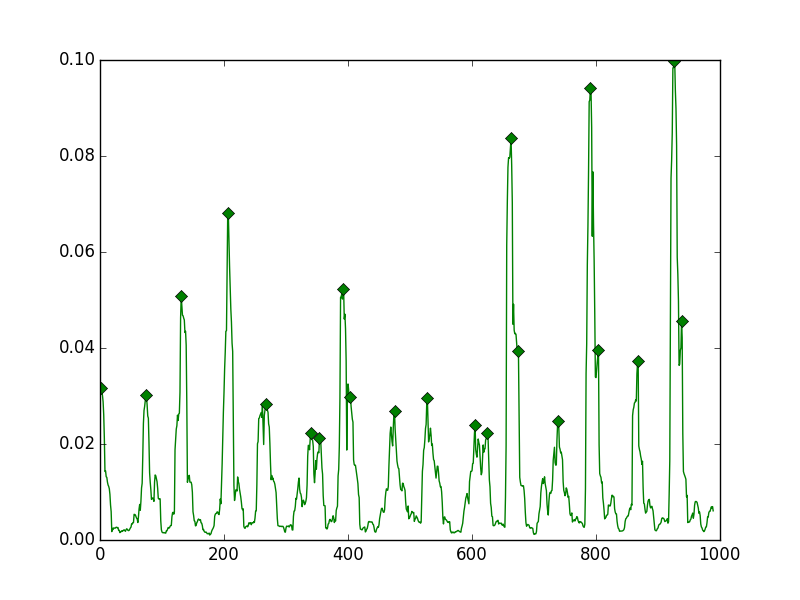
\includegraphics[scale=.50]{figures/608pf}
\caption{Plot of Bhattacharyya distances for the flight on 6/08/16}
\label{fig:tamu-fig1}
\end{figure}

\begin{figure}[h]
\centering
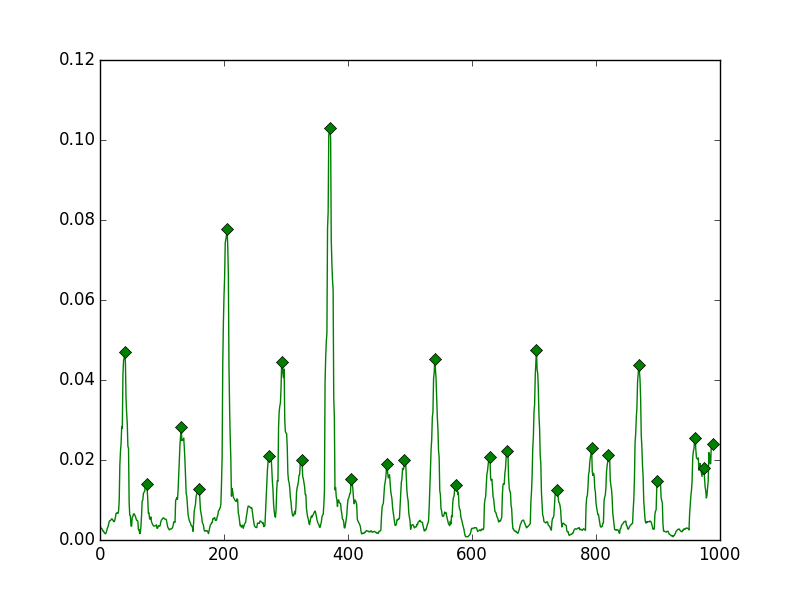
\includegraphics[scale=.50]{figures/629pf}
\caption{Plot of Bhattacharyya distances for the flight on 6/29/16}
\label{fig:tamu-fig2}
\end{figure}

Between both flight datasets, we achieved a detection rate of 66.0\% and a false alarm rate of 24.1\%.
While this is not an acceptable level of performance for the system as a whole, it is effective enough to be useful among a set of features used in a training algorithm.
One reason why this feature does not perform better is that it discards all spatial information in the images; any permutation of the pixels will result in the same pixel distribution.
Furthermore, this feature alone will perform poorly in distinguishing out-of-sync images that happen to be over a homogeneous area, as the pixel distributions will still be close.


\subsection{Other features}

As stated, other features are needed in order to create a robust detection system.
From the field of image processing, there are many image features that can be calculated quickly; our goal is to find features which can be compared and matched among consecutive images in a stream to determine if the images are overlapping by the desired amount.

From previous research into image classification using feature descriptiors \cite{anomalyhyper}, we have identified the SIFT feature as a potential feature which does incorporae spatial information.
This is a scale-invariant feature transform which can be implemented in real time.
Another potential feature with similar attributes is called CenSurE \cite{censure} , which we are also testing.
Other easily computable feature descriptors that we are considering include the BRIEF binary descriptor and the DAISY dense feature description.
The idea with these feature descriptors is to locate a set of keypoints in each image, and then attempt to match them between images to infer that the regions enclosed by matched descriptors are overlapping.

A different feature we are testing is the segmentation and classification of textures within each image using Local Binary Patterns (LBP).
Utilizing the percentage of an image occupied by certain image textures yields a feature similar to the pixel distribution, but over regions of the image rather than on an individual pixel level.
This idea extends naturally into using the multiple bands in multispectral or hyperspectral images for texture classification.


\section {Current efforts}
Our current efforts are split between data gathering and algorithm development.
As mentioned, we have recently gained access to a large amount of raw data for use in this project.
However, the data still needs to be cleaned and labeled before it can be used in algorithm development and assessment.

ALgorithm development has been focused on writing a framework in which we can assess the performance of different image features as well as detection algorithms.
Once the data is prepared, the above mentioned image features will be calculated and used as a feature vector to train and run various learning algorithms.


\subsection{Potential Learning Algorithms}

Among the many supervised learning classification algorithms, we have selected a few that we believe will perform this detection well.
The first among these is logistic regression: one of the most widely used classification algorithms.
Logistic regression takes a labeled training set of feature vectors $\mathbf{x^{(i)}}$ and corresponding binary labels $\mathbf{y^{(i)}}$.
It then finds $\theta$ to minimze the cost function:
\begin{equation}
J(\theta) = \frac{1}{m} \sum_{i=1}^m\frac{1}{2} \left( h_\theta \left( x^{(i)} \right) - y^{(i)} \right)^2
\end{equation}
where $h_\theta (\cdot)$ is the logistic function defined as $h_\theta(x) = \frac{1}{1+e^{-\theta^Tx}}$.

The next learning algorithm we have selected is the backpropagation artificial neural network (ANN).
An ANN is a highly connected directed graphical model, in which the nodes are separated into layers.
In the first layer, called the input layer, your observation or data is input into the layer's nodes.
From here, the information propagates from layer to layer according to the weights of the connections between nodes in each layer.
In training, the output at the final layer is compared to the desired output, and connection weights are adjusted according to the error.
ANNs have massive potential for performing at tasks which are difficult to define or explicity program, but often require a large amount of training data and time to become effective.
The typical neural network diagram is displayed below for clarity.

One of the other possible classification algorithms being considered is the decision tree. 
Since it operates much differently from the other algorithms being considered, the decision tree may prove useful as a point of comparsion.
A decision tree takes a labeled training set of feature vectors $\mathbf{x^{(i)}}$ and corresponding binary labels $\mathbf{y^{(i)}}$, and finds a set of ordered thresholds to compare the features to in order to classify the vector.
This can be visualized as a tree, in which you start at the root node, and move down the tree according to the thresholds defined at the nodes.
Leaf nodes contain the predicted classification.

By comparing the performance of these algorithms, along with the previously mentioned peak-finding, with the image features desired, we believe we can gain a better understanding of the performance of different learning algorithms for this problem, while simultaneously creating a useful system for our intended application.

\begin{figure}[h]
\centering
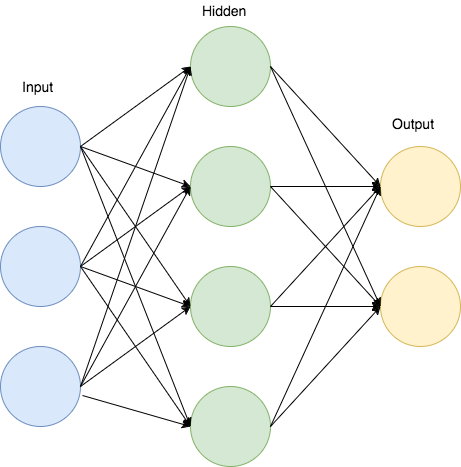
\includegraphics[scale=.50]{figures/NN}
\caption{A general ANN}
\label{fig:tamu-fig3}
\end{figure}




%%%%%%%%%%%%%%%%%%%%%%%%%%%%%%%%%%%%%%%%%%%%%%%%%%%
%
%  New template code for TAMU Theses and Dissertations starting Fall 2016.
%
%  Author: Sean Zachary Roberson
%	 Version 3.16.09
%  Last updated 9/12/2016
%
%%%%%%%%%%%%%%%%%%%%%%%%%%%%%%%%%%%%%%%%%%%%%%%%%%%
%%%%%%%%%%%%%%%%%%%%%%%%%%%%%%%%%%%%%%%%%%%%%%%%%%%%%%%%%%%%%%%%%%%%%%
%%                           SECTION III
%%%%%%%%%%%%%%%%%%%%%%%%%%%%%%%%%%%%%%%%%%%%%%%%%%%%%%%%%%%%%%%%%%%%%



\chapter{RESULTS}

The results of this research are split into the testing of features and learning algorithms, as detailed in the preceding testing methodology.

\section{Feature Evaluation}
As stated previously, plots of the various distances metrics for features are plotted, along with the corresponding labels, to evaluate whether a feature is sufficient.
Shown below are the plots for pixel distribution, BRIEF descriptors, and blob detection.

\subsection{Pixel Distribution}
Shown is the plot for the Bhattacharyya distances between consecutive image pairs for the feature testing subset:

\begin{figure}[h]
\centering
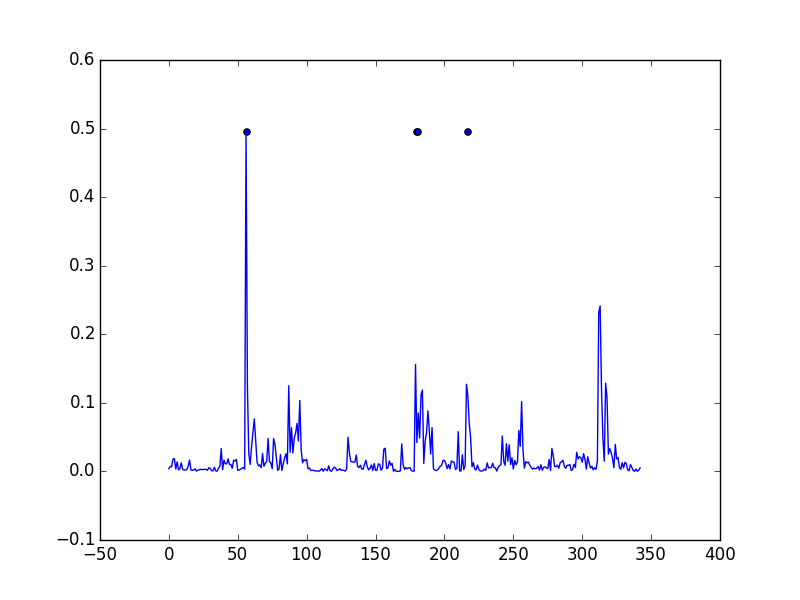
\includegraphics[scale=.50]{figures/611bhattest}
\caption{Pixel distribution evaluation}
\label{fig:tamu-fig3}
\end{figure}

Spikes in the BD can be seen around the locations of the anomalous images, along with some spikes in other areas.

\subsection{BRIEF Descriptors}

First, the plot for the number of BRIEF matches is shown:

\begin{figure}[h]
\centering
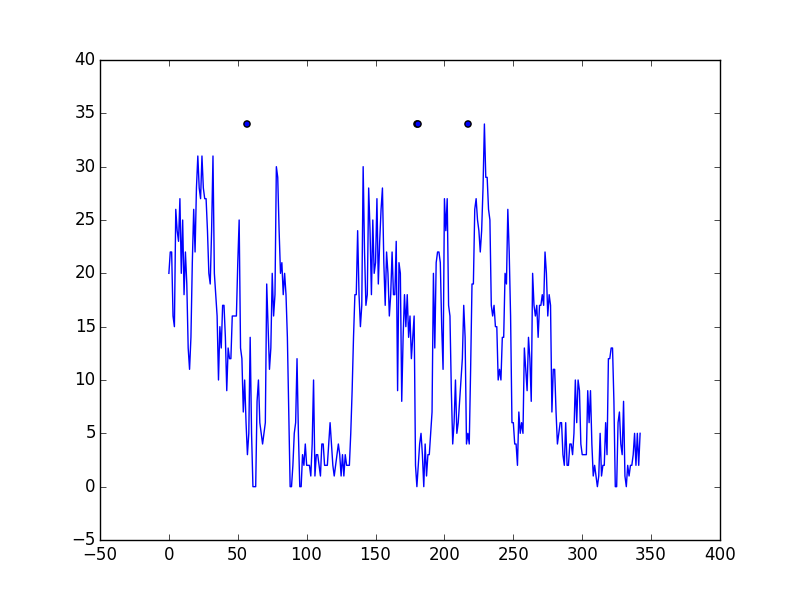
\includegraphics[scale=.50]{figures/611nummatchestest}
\caption{BRIEF number of matches evaluation}
\label{fig:tamu-fig3}
\end{figure}

Next, the plot for the ratio of keypoints matched is shown:

\begin{figure}[h]
\centering
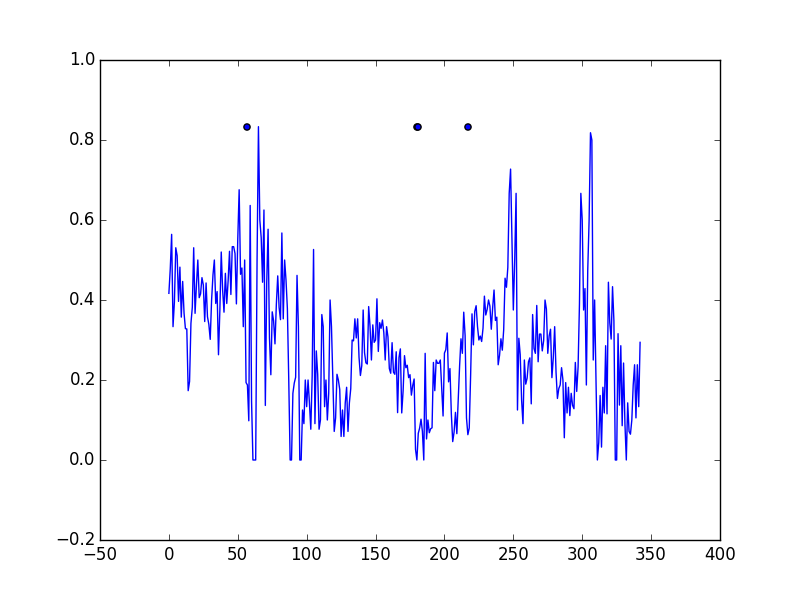
\includegraphics[scale=.50]{figures/611matchratiostest}
\caption{BRIEF keypoint match percentage evaluation}
\label{fig:tamu-fig3}
\end{figure}

Contrary to the other metrics which are true distances, a dip can be seen in the number of matches and the percentage of keypoints matched can be seen around the anomalous images.

\subsection{Blob Detection}

First, the plot for the difference in number of blobs between consecutive images is shown:

\begin{figure}[h]
\centering
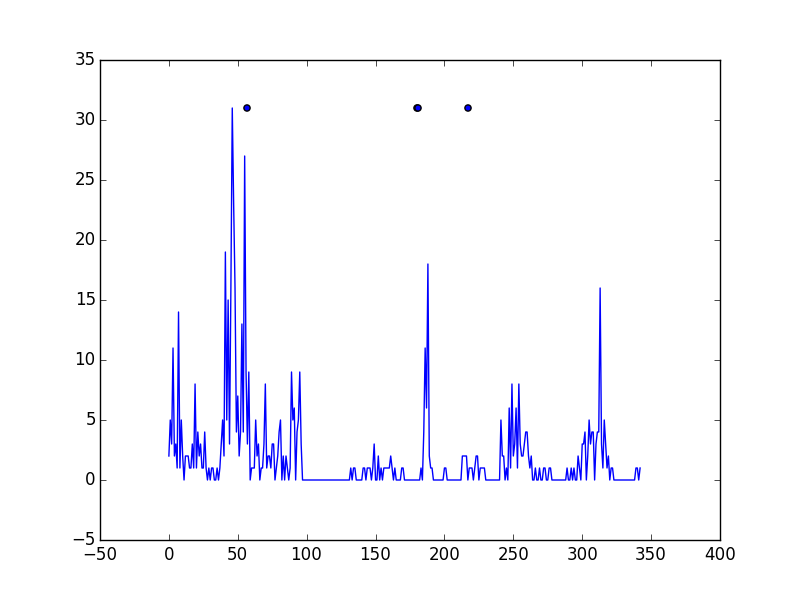
\includegraphics[scale=.50]{figures/blobdiffstest}
\caption{Blob difference evaluation}
\label{fig:tamu-fig3}
\end{figure}

Next, the plot for the difference in total blob area between consecutive images is shown:

\begin{figure}[h]
\centering
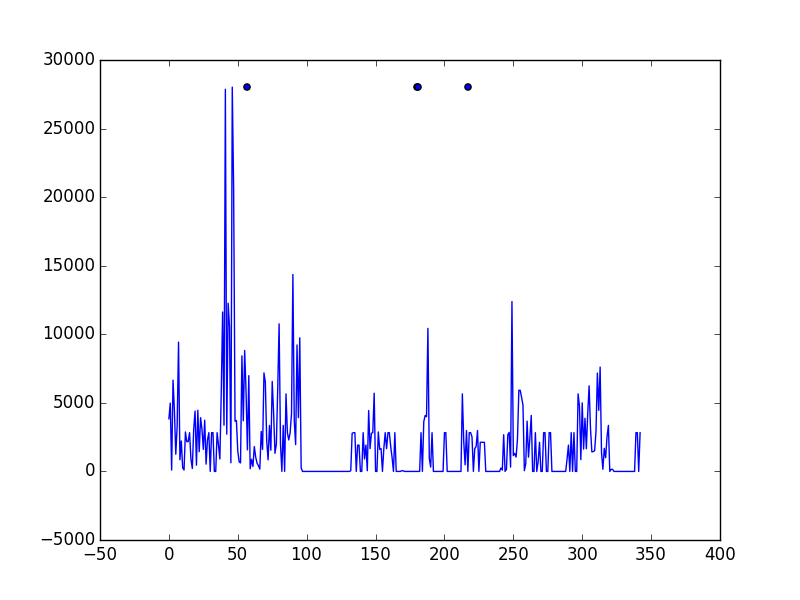
\includegraphics[scale=.50]{figures/blobareadiffstest}
\caption{Blob area difference evaluation}
\label{fig:tamu-fig3}
\end{figure}

Similarly to the distribution distance plots, spikes can be seen around the anomalous images, as well as in other places.

\section{Learning Algorithm Evaluation}

To evaluate the learning algorithms, these distance metrics were concatenated into feature vectors, and fed along with the corresponding label vector to train each algorithm.
As stated in the testing methodology, the models were then tuned to increase performance, and the final averaged values for detection rate, false alarm rate, and overall accuracy are reported in the table below:

\begin{table}[h!]
	\centering
	\begin{tabular}{|l|l|l|l|}
		\hline
		Algorithm & Detection Rate & False Alarm Rate & Overall Accuracy  \\ \hline
		Logistic Regression & 0.956 & 0.077 & 0.933  \\ \hline
		Decision Trees & 0.119 & 0.033 & 0.899  \\ \hline
		Neural Network & 0.75 & 0.038 & 0.959  \\ \hline
		SVM & 0.924 & 0.258  & 0.743 \\ \hline
	\end{tabular}
	\caption{Performance of learning algorithms in anomalous image detection}
\end{table}


The logistic regression model performed the best out of the four algorithms with a 95.6\% detection rate and a 7.7\% false positive rate.
The decision tree predictably performed poorly, as it is a simple model incapable of considering the interaction between features.
The SVM and neural network had decent performance, with the neural network missing 25\% of anomalous image pairs, and the SVM having a fairly high false alarm rate of 25.8\%.

% \section{Yet Another Table}

% Another table is placed here to show the effect of having tables in multiple sections. The list of tables should still double space between table titles, while single spacing long table titles.

% %Fix table labeling.
% \begin{table}[h!]
% 	\centering
% 	\begin{tabular}{|l|l|}
% 		\hline
% 		Dates & Attendance  \\ \hline
% 		August 8-10, 2008 & 3,523  \\ \hline
% 		August 14-16, 2009 & 4,003 \\ \hline
% 		July 9-11, 2010 & 5,049 \\ \hline
% 		August 5-7, 2011 & 6,891  \\ \hline
% 		August 10-12, 2012 & 9,464  \\ \hline
% 		August 16-18, 2013 & 11,077  \\ \hline
% 		July 18-20, 2014 & 14,686 \\ \hline
% 		July 31-August 2, 2015 & 18,411  \\ \hline
% 	\end{tabular}
% 	\caption{San Japan attendance. Data is taken from \cite{ANCONS}. I intentionally make the title of this table long so the single space effect is seen in the list of tables.}
% \end{table}

% You may be wondering why San Japan was chosen. There are a few reasons as to why I did this:

% \begin{enumerate}
% \item It is one of the fastest-growing anime conventions in Texas.
% \item Filler.
% \item I wanted a good variety of table examples.
% \item Because conventions are cool.
% \end{enumerate}



%%%%%%%%%%%%%%%%%%%%%%%%%%%%%%%%%%%%%%%%%%%%%%%%%%%%%%%%%%%%%%%%%%%%%%
%%                           SECTION IV
%%%%%%%%%%%%%%%%%%%%%%%%%%%%%%%%%%%%%%%%%%%%%%%%%%%%%%%%%%%%%%%%%%%%%



\chapter{SUMMARY AND CONCLUSIONS \label{cha:Summary}}

The performance of the selected learning algorithms and features is promising.
All of the selected features proved to be sufficiently discriminating, with the exception of the local binary patterns.
This is understandable, as the feature may be too local to yield much information about the images as a whole.
Furthermore, it is unclear that the texture would necessarily change when images are out of line, or that there could not be significant texture changes in acceptable image pairs, e.g., the entrance of a body of water or a building.

The most promising of the learning algorithms was the logistic regression model, which was able to detect 95.6\% of anomalous images with a false-positive rate of 6.7\%.
The neural network had a very low false-positive rate of 3.8\%, but failed to identify 1/4 of the anomalous images.
As stated in the methodology section, neural networks typically perform better with extremely large training sets, so there is potential for significant improvement with more training data.
The SVM tuning (mainly of the soft margin hyper-parameter) was a balance between a high false-positive rate, and a relatively low detection rate.
Since in our problem it is important to have as high of a detection rate as possible, we chose to increase this at the expense of also increasing the false-positive rate.
The decision tree served its purpose as a point of comparison, but did not perform adequately in comparison to the other models.
It is clear that this problem is not structured in a way that is amenable to tree learning.

With respect to the requirement to have the system run in pseudo real-time, the results are also acceptable, with room for improvement.
All used features are able to be calculated on the order of one second or less, with the total feature vector calculation averaging 1.35 seconds utilizing processing power similar to that of the onboard data processing units.
The imaging systems utilizing in capturing our training and testing data performed imaging at a rate of 40-80 images per minute.
The extraction of all features has the potential to be parallelized for performance increase.
Since the model is not trained onboard the UAV, the model training time is not under any restrictions.
Passing a new feature vector into any of the learning models amounts to a series of simple comparisons or matrix multiplications, the processing time of which is negligible.


Overall, the performance of the system, in particular the logistic regression model, indicates that machine learning is a viable option for the detection of anomalous images in aerial image streams.
A small set of quickly extracted features, along with a model that is trained offline and ported to the onboard computer of a UAV is shown to have potential to alleviate the issue of unchecked anomalous images.


\section{Further Study}
Further study in this area could primarily involve the exploration of even more image features.
As many aerial imaging systems involve multispectral or hyperspectral imagery, a third axis of data could provide opportunity for more revealing 3-dimensional features to be extracted.
In particular, the segmentation of an image by spectral signature could identify differences between bio-matter which appear similar in grayscale.
Beyond this, a full study into the design of a deep neural network trained with larger datasets could potentially yield an even more robust detection system.

Another direction of study would involve extending the classification of anomalies beyond binary.
Anomalies could be classified according to their nature (swinging in various directions, spinning, blur, etc.), or even quantified by how anomalous they are.
This would lead to a multi-class detection system in the case of non-binary classes, and a regression problem in the case of quantified anomalies.


%The next line is the format for inserting new sections.
%Replace the name "newsection"  with the name of your
%new section file.
%\include{data/newsection}

%fix spacing in bibliography, if any...
%%%%%%%%%%%%%%%%%%%%%%%%%%%%%%%%%%%%%%%%%%%%%%%%%%%%%%%%%%%%%
\let\oldbibitem\bibitem
\renewcommand{\bibitem}{\setlength{\itemsep}{0pt}\oldbibitem}
%%%%%%%%%%%%%%%%%%%%%%%%%%%%%%%%%%%%%%%%%%%%%%%%%%%%%%%%%%%%%%%
%The bibliography style declared is the IEEE format. If
%you require a different style, see the document
%bibstyles.pdf included in this package. This file,
%hosted by the University of Vienna, shows several
%bibliography styles and examples of in-text citation
%and a references page.
\bibliographystyle{ieeetr}

\phantomsection
\addcontentsline{toc}{chapter}{REFERENCES}

\renewcommand{\bibname}{{\normalsize\rm REFERENCES}}

%This file is a .bib database that contains the sources.
%This removes the dependency on the previous file
%bibliography.tex.
\bibliography{data/myReference}




%This next line includes appendices. The file
%appendix.tex contains commands pointing to
%the appendix files; be sure to change these
%pointers if you end up changing the filenames.
%Leave this commented if you will not need
%appendix material.
%%%%%%%%%%%%%%%%%%%%%%%%%%%%%%%%%%%%%%%%%%%%%%%%%%%
%
%  New template code for TAMU Theses and Dissertations starting Fall 2016.  
%
%
%  Author: Sean Zachary Roberson 
%	 Version 3.16.09
%  Last updated 9/12/2016
%
%%%%%%%%%%%%%%%%%%%%%%%%%%%%%%%%%%%%%%%%%%%%%%%%%%%

\begin{appendices}
\titleformat{\chapter}{\centering\normalsize}{APPENDIX \thechapter}{0em}{\vskip .5\baselineskip\centering}
\renewcommand{\appendixname}{APPENDIX}

% %%%%%%%%%%%%%%%%%%%%%%%%%%%%%%%%%%%%%%%%%%%%%%%%%%%
%
%  New template code for TAMU Theses and Dissertations starting Fall 2016.
%
%
%  Author: Sean Zachary Roberson 
%	 Version 3.16.09
%  Last updated 9/12/2016
%
%%%%%%%%%%%%%%%%%%%%%%%%%%%%%%%%%%%%%%%%%%%%%%%%%%%

%%%%%%%%%%%%%%%%%%%%%%%%%%%%%%%%%%%%%%%%%%%%%%%%%%%%%%%%%%%%%%%%%%%%%%
%%                           APPENDIX A 
%%%%%%%%%%%%%%%%%%%%%%%%%%%%%%%%%%%%%%%%%%%%%%%%%%%%%%%%%%%%%%%%%%%%%

\phantomsection

\chapter{\uppercase{First Appendix}}

Text for the Appendix follows.

\begin{figure}[h]
\centering
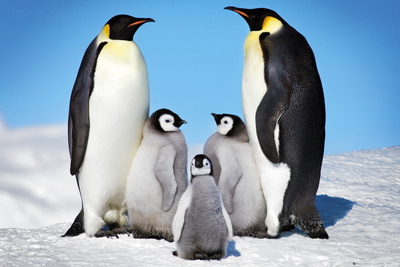
\includegraphics[scale=.50]{figures/Penguins.jpg}
\caption{TAMU figure}
\label{fig:tamu-fig5}
\end{figure}


\end{appendices}


\end{document}
